% 第4章 関連研究
\newpage
%自分の研究との比較が可能なものだけ関連研究に載せる
\renewcommand{\baselinestretch}{1.5}
\section{関連研究}
\renewcommand{\baselinestretch}{1}

\subsection{顕著性マップ生成モデルに関する研究}\label{subsec:itti-kochi}
\par 近年画像解析技術の進歩により風景などの自然画像の顕著性マップ生成モデルに関する研究は多くされているが、ウェブページに特化した顕著性マップ生成モデルに関する研究はほとんど存在しない。

% 自然画像の顕著性マップ
\par 自然画像の顕著性を計算するモデルは昔から研究されて様々なモデルが存在する。中でも基本的な顕著性マップ生成モデルとしてItti-Kochらの顕著性モデル\cite{itti1998model}は広く知られている。このモデルでは、人間の目の視覚認識と同様に色・輝度・方向のそれぞれの視覚特徴を抽出した後に重み付けして足し合わせることにより顕著性マップを生成するモデルである。図\ref{fig_itti-kochi}に計算モデルの構造を示す。このモデルは視覚的顕著性に関連性のある数多くの研究で利用されている。

\begin{figure}[H]
    \centering
    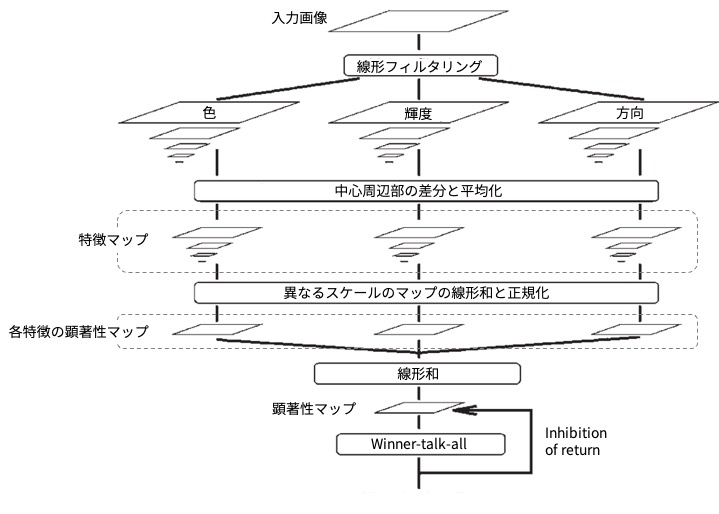
\includegraphics[width=8.5cm]{figures/itti-kochi-model.jpg}
    \caption{Itti-Kochらによる顕著性計算モデルの構造\cite{itti1998model}\label{subsec:itti-kochi}}
    \label{fig_itti-kochi}
\end{figure}

\par また、Kummererらは学習済みのVGG19ニューラルネットワークを使用する事でDeep Gaze 2と呼ばれる自然画像向けの顕著性マップ生成モデルを構築し、MITの顕著性マップのベンチマークであるmit300\cite{mit-saliency-benchmark}のAUCの評価において他のモデルと比較して最も良い精度であることを明らかにした\cite{kummerer2016deepgaze}。

% グラフィックデザインの顕著性マップ
\par 自然画像だけでなくグラフィックデザインに特化した顕著性マップ生成モデルも存在する。Bylinskiiらはポスターなどのグラッフィックデザインとテキストや表が含まれるデータの2種類に分け、それぞれのデータセットを異なる形式で収集してニューラルネットワークモデルを構築することで既存のものと比較して精度の高いグラフィックデザインの顕著性マップを生成可能であることを示している\cite{bylinskii2017learning}。

% ウェブページの顕著性マップ
\par さらにウェブページに特化した顕著性マップ生成モデルも僅かに存在する。人間の注意は大きく分けて色や輝度や方向などの低レベル特徴が主のボトムアップ要因と過去の経験に基づく記憶依存や知識駆動などのトップダウン要因の2つに分けられる。
\par Shenらは従来のボトムアップ要因の顕著性モデルにトップダウン要因を組合せる事で既存のものと比較して精度の高いウェブページの顕著性マップを生成可能であることを示している\cite{shen2014webpage}。彼らは左上の領域が比較的注目されやすい傾向にあるという位置バイアスや人の顔写真に注目が集まりやすいフェイスバイアスをトップダウン要因としてボトムアップ要因とマルチカーネル学習を使用して全ての特徴を統合する事で顕著性マップを生成した。
\par Guptaらはモバイルデバイスとデスクトップデバイスの違いに着目し、スマートフォンの前面カメラを使用して視線を認識し視線データを学習する事で要素レベルでのモバイルUI向け顕著性マップ生成モデルを生成した\cite{Gupta_2018}。

\par しかしながら、いずれの研究においても最終的な出力は顕著性マップのみである。精度が高い顕著性マップを出力しても一目ではどの領域が注目されやすいのか正確に判断する事は難しい。


\subsection{ウェブページの構造分析に関する研究}
% Webページの構造と内容の分析による手法掲載部分の抽出 野中ら
\par 野中らはウェブページの構造を分割するVIPSアルゴリズムの問題点を指摘して、オリジナルの手法でウェブページの構造解析とタグの情報から内容を分析する事で手法掲載箇所の抜き出しを行う手法の提案を行い、従来の手法と比較して有効な結果を得られることを示した\cite{weko_66695_1}。しかし、この手法ではウェブページの重要領域の抜き出しを行う事は出来ない。

% ウェブページの内容・キーワード取得
\par また、Caiらは視覚的表現にもとづいてコンテンツ間の関係を識別する事でウェブコンテンツの構造を抽出する手法を提案し、従来のDOMベースの手法と比較して良い結果が出たことを明らかにしている\cite{cai2003extracting}。しかし、この手法では抽出したレイアウト構造から重要度が高い領域を検出することは出来ない。






% 第5章 本研究の特徴
\newpage
\renewcommand{\baselinestretch}{1.5}
\section{本研究の特徴}
\renewcommand{\baselinestretch}{1}
\par 本研究の特徴は既存の顕著性マップとウェブページの構造を組合せる事で要素単位での顕著性マップである顕著領域マップの生成を行うことと、要素ごとに顕著度を計算してランキング付けを行い顕著度が高い領域をトリミングすることで重要度の高い領域を視覚化する集約図の生成を行うことである。

\subsection{要素単位での顕著性マップの生成}
\par 通常の顕著性マップではグレースケールで顕著性を表現するが、これだけではどの領域が重要度が高いであろうというざっくりとした予想しか行う事ができない。ウェブページを閲覧する際に人は、画像やタイトルやリンクなどタグ単位の要素で重要度を判断する事が多い。そこで本研究では要素単位の顕著性を計算してランキング付けをする事で、正確にどの要素の顕著性が高いのか判断できるウェブページに特化した要素単位の顕著領域マップを生成する事が効果的だと考えた。図\ref{fig_comparesaliency}に早稲田大学ウェブサイトトップページ(2018年12月時点)\cite{waseda_top}のスクリーンショットを入力した時に生成される既存の顕著性マップと提案手法の顕著領域マップの比較を示す。なお、提案手法の顕著領域マップ上の緑色の枠線は特に顕著度が高い重要領域10箇所を表している。

\begin{figure}[H]
    \centering
    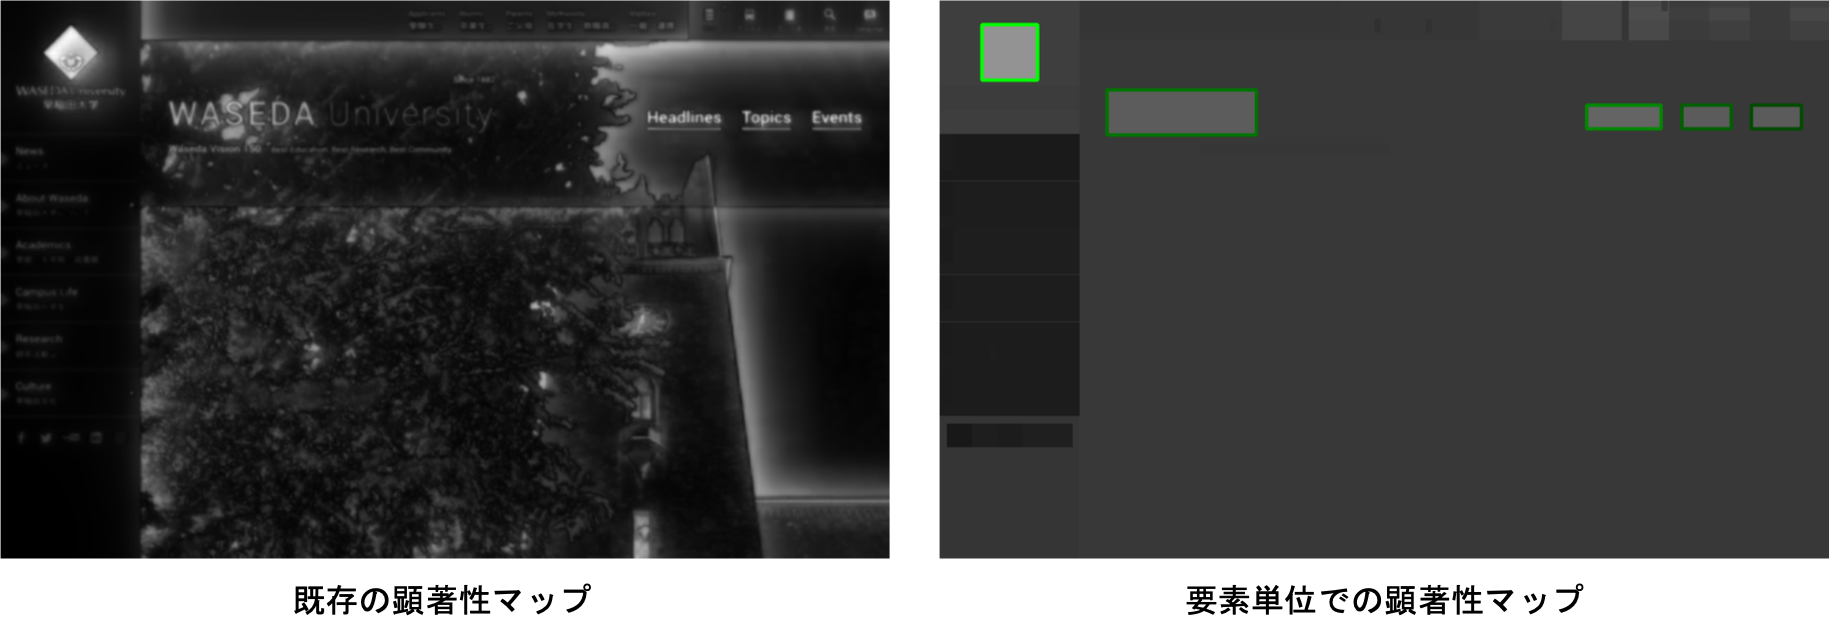
\includegraphics[width=12cm]{figures/example-originalsaliencymap.png}
    \caption{既存の顕著性マップと要素単位での顕著性マップとの比較}
    \label{fig_comparesaliency}
\end{figure}

\subsection{重要領域の視覚化}
\par ウェブページの顕著領域にはウェブページの重要な内容が含まれる事が多い。既存の研究では精度の高い顕著性マップの生成を行う事で研究が完結している事がほとんどである。しかしながら、要素ごとの顕著性を計算する事で作成した顕著度ランキングを元に重要領域ををタイル状に並べて一つの画像にまとめる事でウェブページの内容を簡単に把握可能な集約図を生成出来ると考えた。これにより、ネットユーザーが初見のウェブページにアクセスした際の内容把握の時間短縮に繋がる可能性がある。図\ref{fig_imoortanceregion}に早稲田大学ウェブサイトトップページ(2018年12月時点)\cite{waseda_top}の重要領域を集約した集約図を示す。

\begin{figure}[H]
    \centering
    
\includegraphics[width=8cm]{figures/example-importanceregion.png}
    \caption{生成された集約図の例}
    \label{fig_imoortanceregion}
\end{figure}
